\begin{figure}[]
     \centering
     \begin{subfigure}[b]{0.48\textwidth}
         \centering
         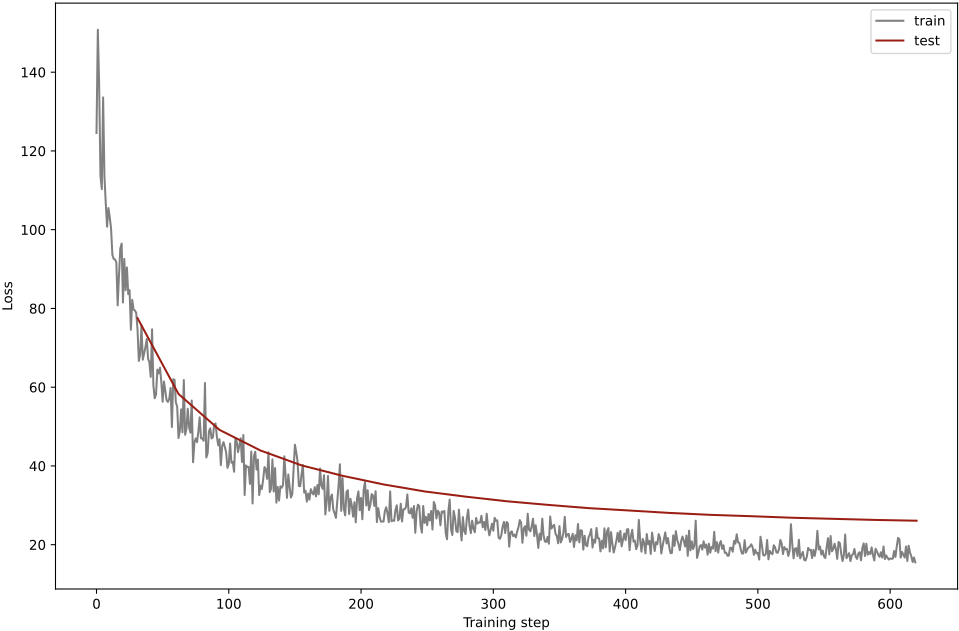
\includegraphics[width=\textwidth]{observational/img/bnn/sigmas/LC_s0.1_s1e-06.png}
         \caption{Loss; $\sigma_1=1*10^{-1}$, $\sigma_2=1*10^{-6}$}
     \end{subfigure}
     \hfill
     \begin{subfigure}[b]{0.48\textwidth}
         \centering
         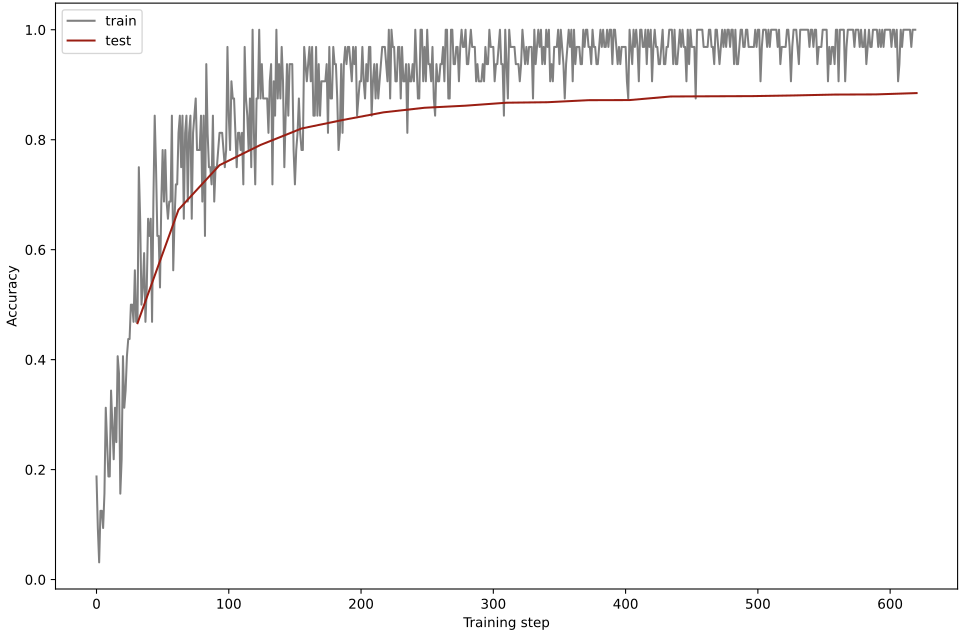
\includegraphics[width=\textwidth]{observational/img/bnn/sigmas/AC_s0.1_s1e-06.png}
         \caption{Accuracy; $\sigma_1=1*10^{-1}$, $\sigma_2=1*10^{-6}$}
     \end{subfigure} 
     \par\bigskip
     \begin{subfigure}[b]{0.48\textwidth}
         \centering
         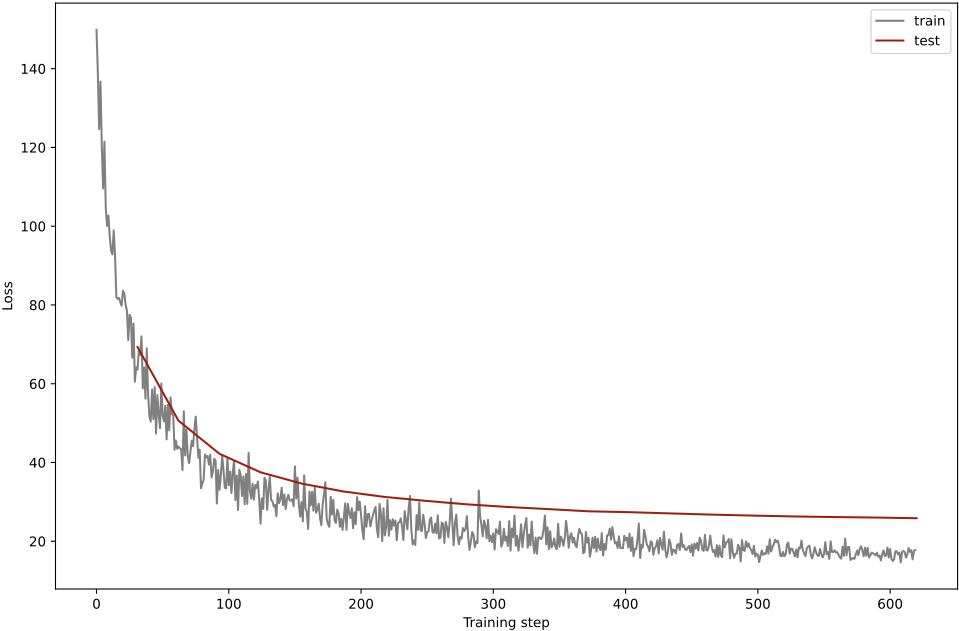
\includegraphics[width=\textwidth]{observational/img/bnn/sigmas/LC_s0.5_s1e-06.png}
         \caption{Loss; $\sigma_1=5*10^{-1}$, $\sigma_2=1*10^{-6}$}
     \end{subfigure}
     \hfill
     \begin{subfigure}[b]{0.48\textwidth}
         \centering
         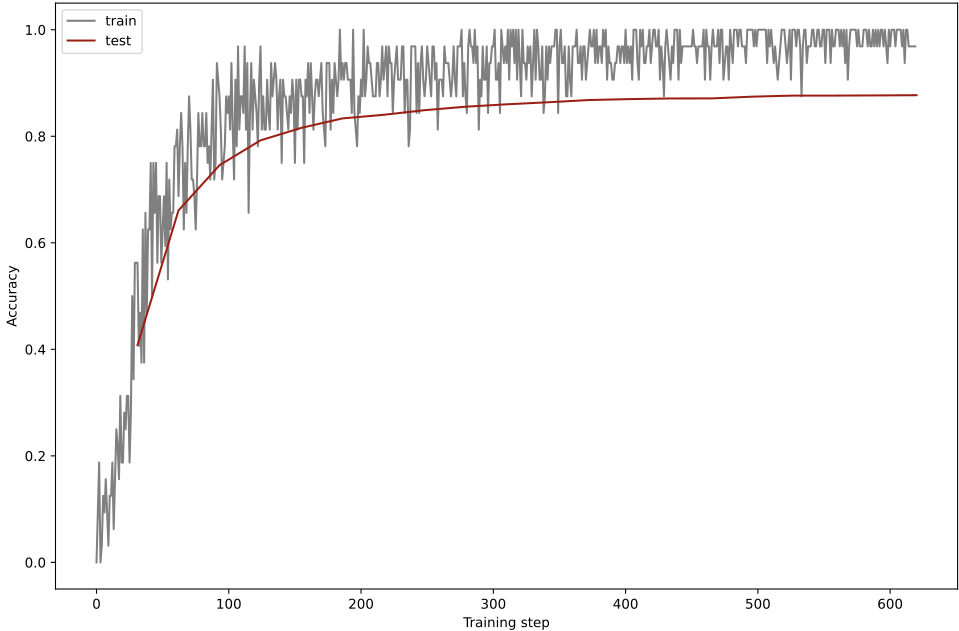
\includegraphics[width=\textwidth]{observational/img/bnn/sigmas/AC_s0.5_s1e-06.png}
         \caption{Accuracy; $\sigma_1=5*10^{-1}$, $\sigma_2=1*10^{-6}$}
     \end{subfigure} 
     \par\bigskip
     \begin{subfigure}[b]{0.48\textwidth}
         \centering
         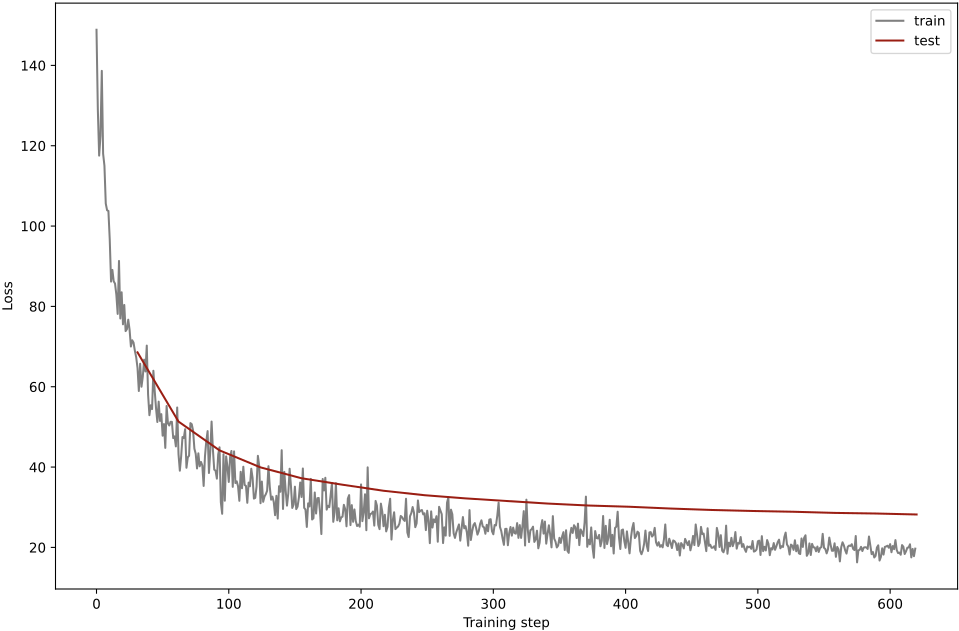
\includegraphics[width=\textwidth]{observational/img/bnn/sigmas/LC_default.png}
         \caption{Loss; $\sigma_1=1$, $\sigma_2=1*10^{-6}$}
     \end{subfigure}
     \hfill
     \begin{subfigure}[b]{0.48\textwidth}
         \centering
         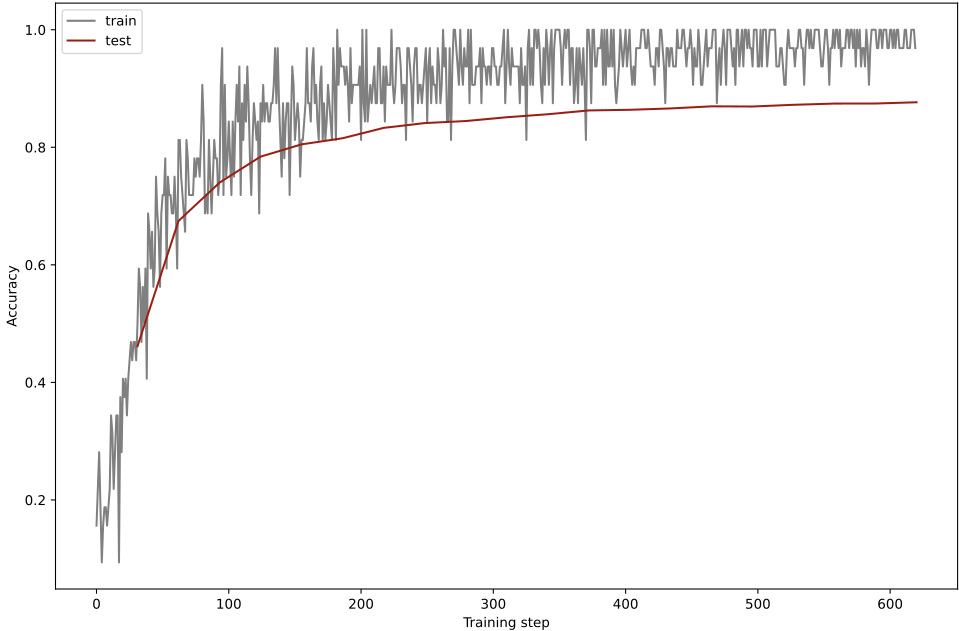
\includegraphics[width=\textwidth]{observational/img/bnn/sigmas/AC_default.png}
         \caption{Accuracy; $\sigma_1=1$, $\sigma_2=1*10^{-6}$}
     \end{subfigure}
     \caption[Sigma values influence on the BNN learning process]{Sigma values influence on the Bayesian Neural Network learning process.}
    \label{fig:bnn-sigmas}
\end{figure}
\begin{figure}[]\ContinuedFloat
    \begin{subfigure}[b]{0.48\textwidth}\ContinuedFloat
         \centering
         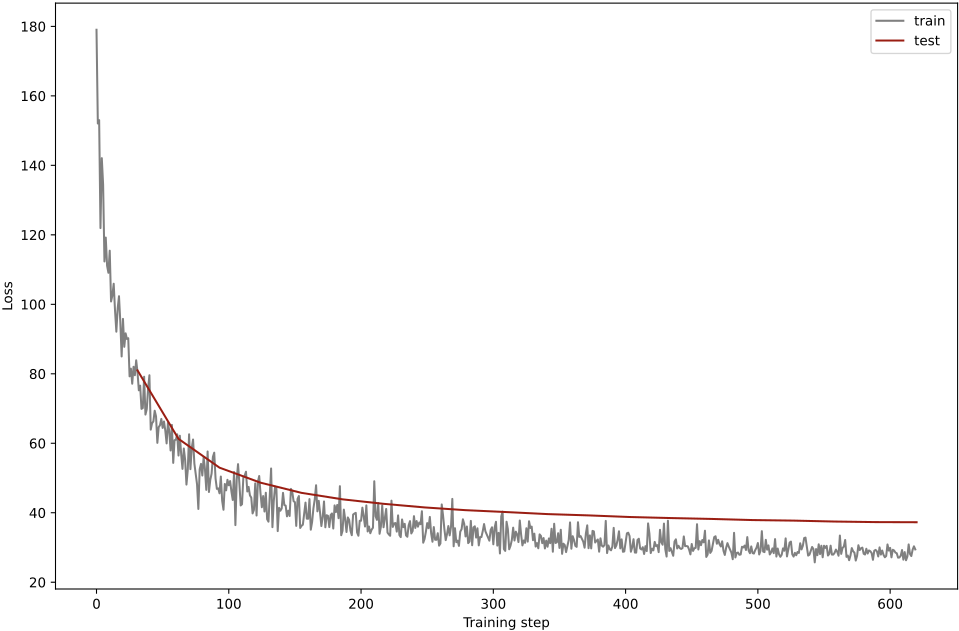
\includegraphics[width=\textwidth]{observational/img/bnn/sigmas/LC_s10_s1e-06.png}
         \caption{Loss; $\sigma_1=1*10^{1}$, $\sigma_2=1*10^{-6}$}
     \end{subfigure}
     \hfill
     \begin{subfigure}[b]{0.48\textwidth}
         \centering
         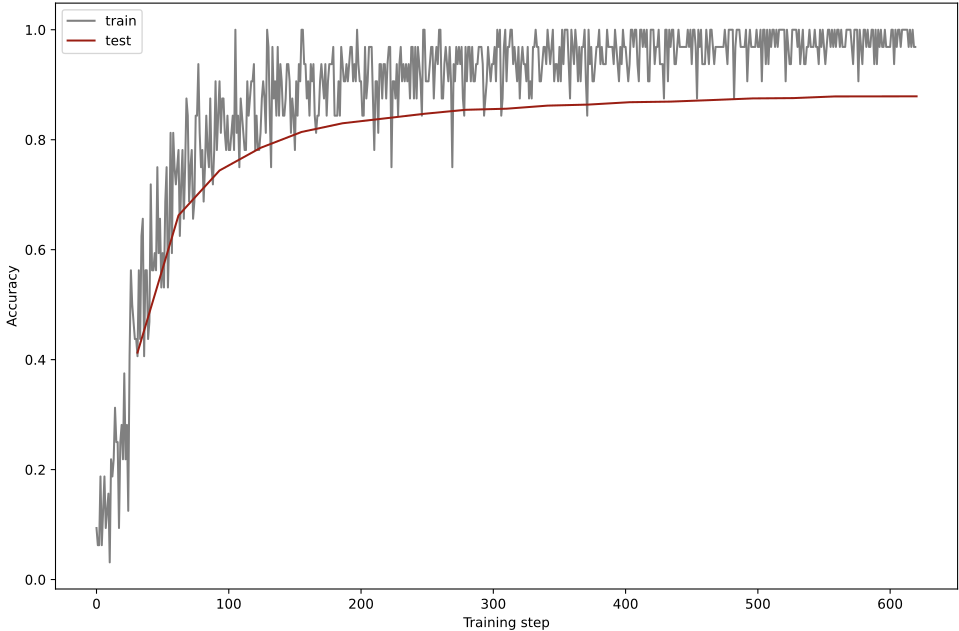
\includegraphics[width=\textwidth]{observational/img/bnn/sigmas/AC_s10_s1e-06.png}
         \caption{Accuracy; $\sigma_1=1*10^{1}$, $\sigma_2=1*10^{-6}$}
     \end{subfigure} 
     \par\bigskip
     \begin{subfigure}[b]{0.48\textwidth}
         \centering
         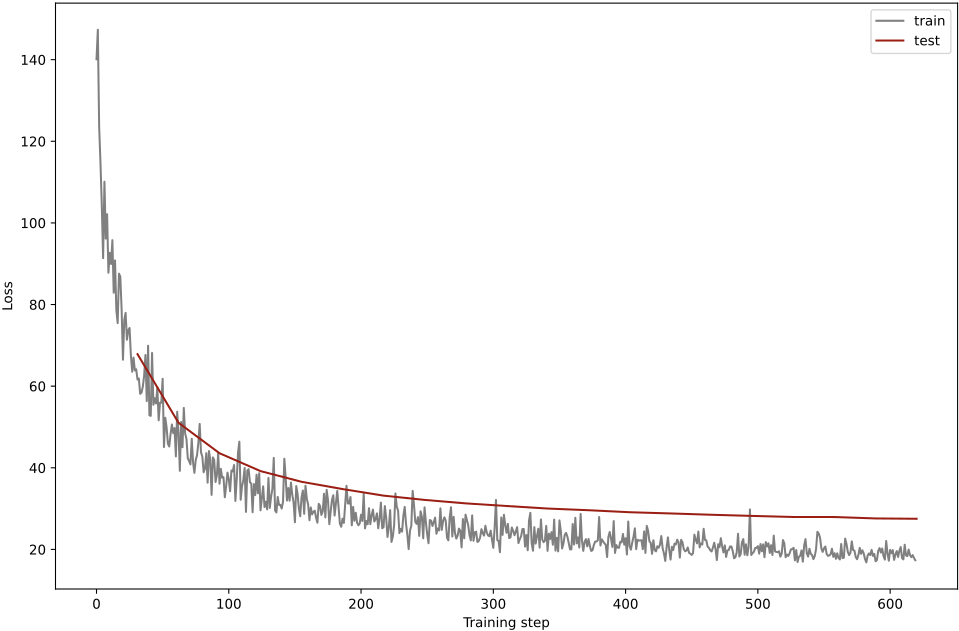
\includegraphics[width=\textwidth]{observational/img/bnn/sigmas/LC_s1_s0.001.png}
         \caption{Loss; $\sigma_1=1$, $\sigma_2=1*10^{-3}$}
     \end{subfigure}
     \hfill
     \begin{subfigure}[b]{0.48\textwidth}
         \centering
         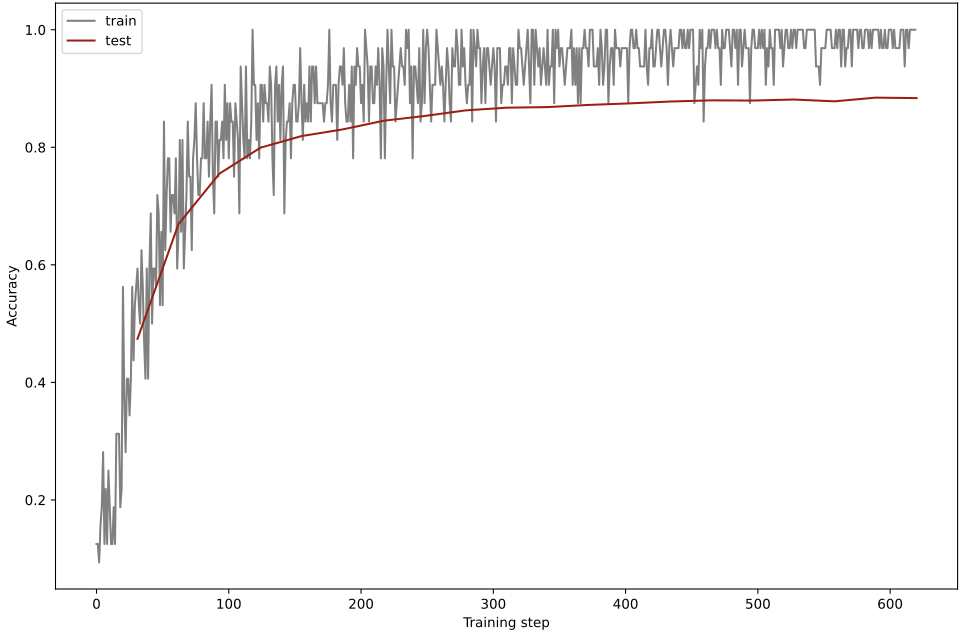
\includegraphics[width=\textwidth]{observational/img/bnn/sigmas/AC_s1_s0.001.png}
         \caption{Accuracy; $\sigma_1=1$, $\sigma_2=1*10^{-3}$}
     \end{subfigure}
     \caption*{Sigma values influence on the Bayesian Neural Network learning process (cont.)}
\end{figure}